\chapter{A Signed Statement}

Noirtier was prepared to receive them, dressed in black, and installed
in his armchair. When the three persons he expected had entered, he
looked at the door, which his valet immediately closed.

“Listen,” whispered Villefort to Valentine, who could not conceal her
joy; “if M. Noirtier wishes to communicate anything which would delay
your marriage, I forbid you to understand him.”

Valentine blushed, but did not answer. Villefort, approached Noirtier.

“Here is M. Franz d’Épinay,” said he; “you requested to see him. We
have all wished for this interview, and I trust it will convince you
how ill-formed are your objections to Valentine’s marriage.”

Noirtier answered only by a look which made Villefort’s blood run cold.
He motioned to Valentine to approach. In a moment, thanks to her habit
of conversing with her grandfather, she understood that he asked for a
key. Then his eye was fixed on the drawer of a small chest between the
windows. She opened the drawer, and found a key; and, understanding
that was what he wanted, again watched his eyes, which turned toward an
old secretaire which had been neglected for many years and was supposed
to contain nothing but useless documents.

“Shall I open the secretaire?” asked Valentine.

“Yes,” said the old man.

“And the drawers?”

“Yes.”

“Those at the side?”

“No.”

“The middle one?”

“Yes.”

Valentine opened it and drew out a bundle of papers. “Is that what you
wish for?” asked she.

“No.”

She took successively all the other papers out till the drawer was
empty. “But there are no more,” said she. Noirtier’s eye was fixed on
the dictionary.

“Yes, I understand, grandfather,” said the young girl.

\begin{figure}[ht]
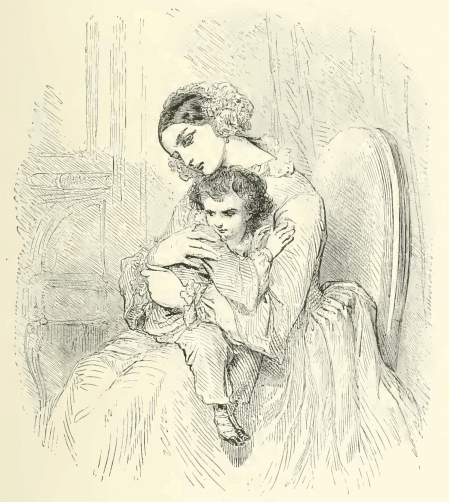
\includegraphics[width=\textwidth]{40036m.jpg}
\end{figure}

She pointed to each letter of the alphabet. At the letter S the old man
stopped her. She opened, and found the word “secret.”

“Ah! is there a secret spring?” said Valentine.

“Yes,” said Noirtier.

“And who knows it?” Noirtier looked at the door where the servant had
gone out.

“Barrois?” said she.

“Yes.”

“Shall I call him?”

“Yes.”

Valentine went to the door, and called Barrois. Villefort’s impatience
during this scene made the perspiration roll from his forehead, and
Franz was stupefied. The old servant came.

“Barrois,” said Valentine, “my grandfather has told me to open that
drawer in the secretaire, but there is a secret spring in it, which you
know—will you open it?”

Barrois looked at the old man. “Obey,” said Noirtier’s intelligent eye.
Barrois touched a spring, the false bottom came out, and they saw a
bundle of papers tied with a black string.

“Is that what you wish for?” said Barrois.

“Yes.”

“Shall I give these papers to M. de Villefort?”

“No.”

“To Mademoiselle Valentine?”

“No.”

“To M. Franz d’Épinay?”

“Yes.”

Franz, astonished, advanced a step. “To me, sir?” said he.

“Yes.”

Franz took them from Barrois and casting a glance at the cover, read:

“‘To be given, after my death, to General Durand, who shall bequeath
the packet to his son, with an injunction to preserve it as containing
an important document.’

“Well, sir,” asked Franz, “what do you wish me to do with this paper?”

“To preserve it, sealed up as it is, doubtless,” said the procureur.

“No,” replied Noirtier eagerly.

“Do you wish him to read it?” said Valentine.

“Yes,” replied the old man.

“You understand, baron, my grandfather wishes you to read this paper,”
said Valentine.

“Then let us sit down,” said Villefort impatiently, “for it will take
some time.”

“Sit down,” said the old man. Villefort took a chair, but Valentine
remained standing by her father’s side, and Franz before him, holding
the mysterious paper in his hand. “Read,” said the old man. Franz
untied it, and in the midst of the most profound silence read:

\begin{figure}[ht]
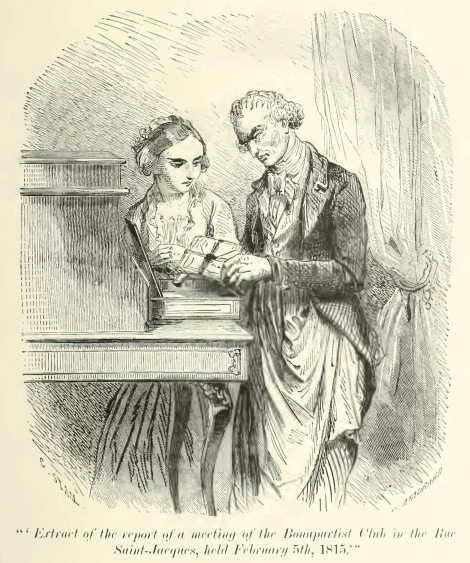
\includegraphics[width=\textwidth]{40038m.jpg}
\end{figure}

“‘\textit{Extract of the report of a meeting of the Bonapartist Club in the
Rue Saint-Jacques, held February 5th, 1815}.’”

Franz stopped. “February 5th, 1815!” said he; “it is the day my father
was murdered.” Valentine and Villefort were dumb; the eye of the old
man alone seemed to say clearly, “Go on.”

“But it was on leaving this club,” said he, “my father disappeared.”

Noirtier’s eye continued to say, “Read.” He resumed:—

“‘The undersigned Louis-Jacques Beaurepaire, lieutenant-colonel of
artillery, Étienne Duchampy, general of brigade, and Claude Lecharpal,
keeper of woods and forests, declare, that on the 4th of February, a
letter arrived from the Island of Elba, recommending to the kindness
and the confidence of the Bonapartist Club, General Flavien de Quesnel,
who having served the emperor from 1804 to 1814 was supposed to be
devoted to the interests of the Napoleon dynasty, notwithstanding the
title of baron which Louis XVIII. had just granted to him with his
estate of Épinay.

\begin{figure}[ht]
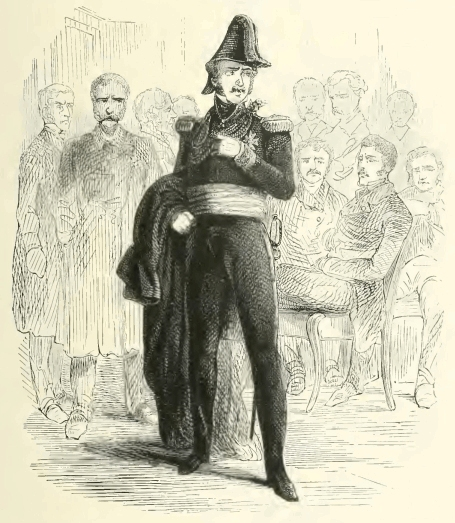
\includegraphics[width=\textwidth]{40040m.jpg}
\end{figure}

“‘A note was in consequence addressed to General de Quesnel, begging
him to be present at the meeting next day, the 5th. The note indicated
neither the street nor the number of the house where the meeting was to
be held; it bore no signature, but it announced to the general that
someone would call for him if he would be ready at nine o’clock. The
meetings were always held from that time till midnight. At nine o’clock
the president of the club presented himself; the general was ready, the
president informed him that one of the conditions of his introduction
was that he should be eternally ignorant of the place of meeting, and
that he would allow his eyes to be bandaged, swearing that he would not
endeavor to take off the bandage. General de Quesnel accepted the
condition, and promised on his honor not to seek to discover the road
they took. The general’s carriage was ready, but the president told him
it was impossible for him to use it, since it was useless to blindfold
the master if the coachman knew through what streets he went. “What
must be done then?” asked the general.—“I have my carriage here,” said
the president.

“‘“Have you, then, so much confidence in your servant that you can
intrust him with a secret you will not allow me to know?”

“‘“Our coachman is a member of the club,” said the president; “we shall
be driven by a State-Councillor.”

“‘“Then we run another risk,” said the general, laughing, “that of
being upset.” We insert this joke to prove that the general was not in
the least compelled to attend the meeting, but that he came willingly.
When they were seated in the carriage the president reminded the
general of his promise to allow his eyes to be bandaged, to which he
made no opposition. On the road the president thought he saw the
general make an attempt to remove the handkerchief, and reminded him of
his oath. “Sure enough,” said the general. The carriage stopped at an
alley leading out of the Rue Saint-Jacques. The general alighted,
leaning on the arm of the president, of whose dignity he was not aware,
considering him simply as a member of the club; they went through the
alley, mounted a flight of stairs, and entered the assembly-room.

“‘The deliberations had already begun. The members, apprised of the
sort of presentation which was to be made that evening, were all in
attendance. When in the middle of the room the general was invited to
remove his bandage, he did so immediately, and was surprised to see so
many well-known faces in a society of whose existence he had till then
been ignorant. They questioned him as to his sentiments, but he
contented himself with answering, that the letters from the Island of
Elba ought to have informed them——’”

Franz interrupted himself by saying, “My father was a royalist; they
need not have asked his sentiments, which were well known.”

“And hence,” said Villefort, “arose my affection for your father, my
dear M. Franz. Opinions held in common are a ready bond of union.”

“Read again,” said the old man.

Franz continued:

“‘The president then sought to make him speak more explicitly, but M.
de Quesnel replied that he wished first to know what they wanted with
him. He was then informed of the contents of the letter from the Island
of Elba, in which he was recommended to the club as a man who would be
likely to advance the interests of their party. One paragraph spoke of
the return of Bonaparte and promised another letter and further
details, on the arrival of the \textit{Pharaon} belonging to the shipbuilder
Morrel, of Marseilles, whose captain was entirely devoted to the
emperor. During all this time, the general, on whom they thought to
have relied as on a brother, manifested evidently signs of discontent
and repugnance. When the reading was finished, he remained silent, with
knitted brows.

“‘“Well,” asked the president, “what do you say to this letter,
general?”

“‘“I say that it is too soon after declaring myself for Louis XVIII. to
break my vow in behalf of the ex-emperor.” This answer was too clear to
permit of any mistake as to his sentiments. “General,” said the
president, “we acknowledge no King Louis XVIII., or an ex-emperor, but
his majesty the emperor and king, driven from France, which is his
kingdom, by violence and treason.”

“‘“Excuse me, gentlemen,” said the general; “you may not acknowledge
Louis XVIII., but I do, as he has made me a baron and a field-marshal,
and I shall never forget that for these two titles I am indebted to his
happy return to France.”

“‘“Sir,” said the president, rising with gravity, “be careful what you
say; your words clearly show us that they are deceived concerning you
in the Island of Elba, and have deceived us! The communication has been
made to you in consequence of the confidence placed in you, and which
does you honor. Now we discover our error; a title and promotion attach
you to the government we wish to overturn. We will not constrain you to
help us; we enroll no one against his conscience, but we will compel
you to act generously, even if you are not disposed to do so.”

“‘“You would call acting generously, knowing your conspiracy and not
informing against you, that is what I should call becoming your
accomplice. You see I am more candid than you.”’”

“Ah, my father!” said Franz, interrupting himself. “I understand now
why they murdered him.” Valentine could not help casting one glance
towards the young man, whose filial enthusiasm it was delightful to
behold. Villefort walked to and fro behind them. Noirtier watched the
expression of each one, and preserved his dignified and commanding
attitude. Franz returned to the manuscript, and continued:

“‘“Sir,” said the president, “you have been invited to join this
assembly—you were not forced here; it was proposed to you to come
blindfolded—you accepted. When you complied with this twofold request
you well knew we did not wish to secure the throne of Louis XVIII., or
we should not take so much care to avoid the vigilance of the police.
It would be conceding too much to allow you to put on a mask to aid you
in the discovery of our secret, and then to remove it that you may ruin
those who have confided in you. No, no, you must first say if you
declare yourself for the king of a day who now reigns, or for his
majesty the emperor.”

“‘“I am a royalist,” replied the general; “I have taken the oath of
allegiance to Louis XVIII., and I will adhere to it.” These words were
followed by a general murmur, and it was evident that several of the
members were discussing the propriety of making the general repent of
his rashness.

“‘The president again arose, and having imposed silence, said,—“Sir,
you are too serious and too sensible a man not to understand the
consequences of our present situation, and your candor has already
dictated to us the conditions which remain for us to offer you.” The
general, putting his hand on his sword, exclaimed,—“If you talk of
honor, do not begin by disavowing its laws, and impose nothing by
violence.”

“‘“And you, sir,” continued the president, with a calmness still more
terrible than the general’s anger, “I advise you not to touch your
sword.” The general looked around him with slight uneasiness; however
he did not yield, but calling up all his fortitude, said,—“I will not
swear.”

“‘“Then you must die,” replied the president calmly. M. d’Épinay became
very pale; he looked round him a second time, several members of the
club were whispering, and getting their arms from under their cloaks.
“General,” said the president, “do not alarm yourself; you are among
men of honor who will use every means to convince you before resorting
to the last extremity, but as you have said, you are among
conspirators, you are in possession of our secret, and you must restore
it to us.” A significant silence followed these words, and as the
general did not reply,—“Close the doors,” said the president to the
door-keeper.

\begin{figure}[ht]
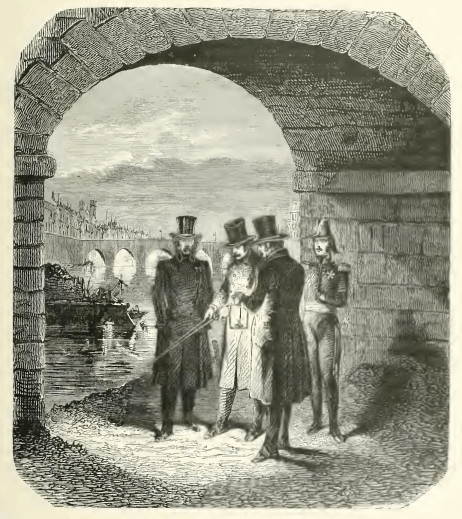
\includegraphics[width=\textwidth]{40042m.jpg}
\end{figure}

“‘The same deadly silence succeeded these words. Then the general
advanced, and making a violent effort to control his feelings,—“I have
a son,” said he, “and I ought to think of him, finding myself among
assassins.”

“‘“General,” said the chief of the assembly, “one man may insult
fifty—it is the privilege of weakness. But he does wrong to use his
privilege. Follow my advice, swear, and do not insult.” The general,
again daunted by the superiority of the chief, hesitated a moment; then
advancing to the president’s desk,—“What is the form, said he.

“‘“It is this:—‘I swear by my honor not to reveal to anyone what I have
seen and heard on the 5th of February, 1815, between nine and ten
o’clock in the evening; and I plead guilty of death should I ever
violate this oath.’” The general appeared to be affected by a nervous
tremor, which prevented his answering for some moments; then,
overcoming his manifest repugnance, he pronounced the required oath,
but in so low a tone as to be scarcely audible to the majority of the
members, who insisted on his repeating it clearly and distinctly, which
he did.

“‘“Now am I at liberty to retire?” said the general. The president
rose, appointed three members to accompany him, and got into the
carriage with the general after bandaging his eyes. One of those three
members was the coachman who had driven them there. The other members
silently dispersed. “Where do you wish to be taken?” asked the
president.—“Anywhere out of your presence,” replied M. d’Épinay.
“Beware, sir,” replied the president, “you are no longer in the
assembly, and have only to do with individuals; do not insult them
unless you wish to be held responsible.” But instead of listening, M.
d’Épinay went on,—“You are still as brave in your carriage as in your
assembly because you are still four against one.” The president stopped
the coach. They were at that part of the Quai des Ormes where the steps
lead down to the river. “Why do you stop here?” asked d’Épinay.

“‘“Because, sir,” said the president, “you have insulted a man, and
that man will not go one step farther without demanding honorable
reparation.”

“‘“Another method of assassination?” said the general, shrugging his
shoulders.

“‘“Make no noise, sir, unless you wish me to consider you as one of the
men of whom you spoke just now as cowards, who take their weakness for
a shield. You are alone, one alone shall answer you; you have a sword
by your side, I have one in my cane; you have no witness, one of these
gentlemen will serve you. Now, if you please, remove your bandage.” The
general tore the handkerchief from his eyes. “At last,” said he, “I
shall know with whom I have to do.” They opened the door and the four
men alighted.’”

Franz again interrupted himself, and wiped the cold drops from his
brow; there was something awful in hearing the son read aloud in
trembling pallor these details of his father’s death, which had
hitherto been a mystery. Valentine clasped her hands as if in prayer.
Noirtier looked at Villefort with an almost sublime expression of
contempt and pride.

Franz continued:

“‘It was, as we said, the fifth of February. For three days the mercury
had been five or six degrees below freezing and the steps were covered
with ice. The general was stout and tall, the president offered him the
side of the railing to assist him in getting down. The two witnesses
followed. It was a dark night. The ground from the steps to the river
was covered with snow and hoarfrost, the water of the river looked
black and deep. One of the seconds went for a lantern in a coal-barge
near, and by its light they examined the weapons. The president’s
sword, which was simply, as he had said, one he carried in his cane,
was five inches shorter than the general’s, and had no guard. The
general proposed to cast lots for the swords, but the president said it
was he who had given the provocation, and when he had given it he had
supposed each would use his own arms. The witnesses endeavored to
insist, but the president bade them be silent. The lantern was placed
on the ground, the two adversaries took their stations, and the duel
began. The light made the two swords appear like flashes of lightning;
as for the men, they were scarcely perceptible, the darkness was so
great.

\begin{figure}[ht]
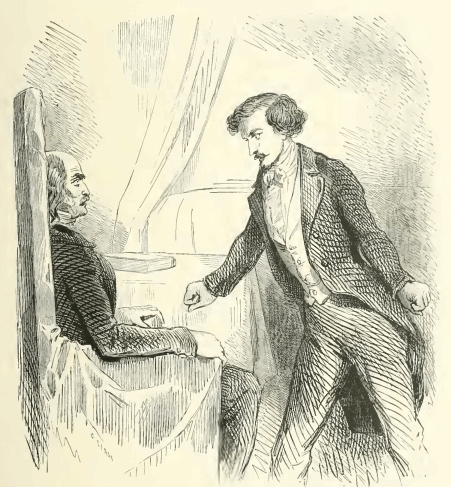
\includegraphics[width=\textwidth]{40044m.jpg}
\end{figure}

“‘General d’Épinay passed for one of the best swordsmen in the army,
but he was pressed so closely in the onset that he missed his aim and
fell. The witnesses thought he was dead, but his adversary, who knew he
had not struck him, offered him the assistance of his hand to rise. The
circumstance irritated instead of calming the general, and he rushed on
his adversary. But his opponent did not allow his guard to be broken.
He received him on his sword and three times the general drew back on
finding himself too closely engaged, and then returned to the charge.
At the third he fell again. They thought he slipped, as at first, and
the witnesses, seeing he did not move, approached and endeavored to
raise him, but the one who passed his arm around the body found it was
moistened with blood. The general, who had almost fainted, revived.
“Ah,” said he, “they have sent some fencing-master to fight with me.”
The president, without answering, approached the witness who held the
lantern, and raising his sleeve, showed him two wounds he had received
in his arm; then opening his coat, and unbuttoning his waistcoat,
displayed his side, pierced with a third wound. Still he had not even
uttered a sigh. General d’Épinay died five minutes after.’”

Franz read these last words in a voice so choked that they were hardly
audible, and then stopped, passing his hand over his eyes as if to
dispel a cloud; but after a moment’s silence, he continued:

“‘The president went up the steps, after pushing his sword into his
cane; a track of blood on the snow marked his course. He had scarcely
arrived at the top when he heard a heavy splash in the water—it was the
general’s body, which the witnesses had just thrown into the river
after ascertaining that he was dead. The general fell, then, in a loyal
duel, and not in ambush as it might have been reported. In proof of
this we have signed this paper to establish the truth of the facts,
lest the moment should arrive when either of the actors in this
terrible scene should be accused of premeditated murder or of
infringement of the laws of honor.

“‘Signed, Beaurepaire, Duchampy, and Lecharpal.’”

When Franz had finished reading this account, so dreadful for a son;
when Valentine, pale with emotion, had wiped away a tear; when
Villefort, trembling, and crouched in a corner, had endeavored to
lessen the storm by supplicating glances at the implacable old man,—

“Sir,” said d’Épinay to Noirtier, “since you are well acquainted with
all these details, which are attested by honorable signatures,—since
you appear to take some interest in me, although you have only
manifested it hitherto by causing me sorrow, refuse me not one final
satisfaction—tell me the name of the president of the club, that I may
at least know who killed my father.”

Villefort mechanically felt for the handle of the door; Valentine, who
understood sooner than anyone her grandfather’s answer, and who had
often seen two scars upon his right arm, drew back a few steps.

“Mademoiselle,” said Franz, turning towards Valentine, “unite your
efforts with mine to find out the name of the man who made me an orphan
at two years of age.” Valentine remained dumb and motionless.

“Hold, sir,” said Villefort, “do not prolong this dreadful scene. The
names have been purposely concealed; my father himself does not know
who this president was, and if he knows, he cannot tell you; proper
names are not in the dictionary.”

“Oh, misery,” cried Franz: “the only hope which sustained me and
enabled me to read to the end was that of knowing, at least, the name
of him who killed my father! Sir, sir,” cried he, turning to Noirtier,
“do what you can—make me understand in some way!”

“Yes,” replied Noirtier.

“Oh, mademoiselle, mademoiselle!” cried Franz, “your grandfather says
he can indicate the person. Help me,—lend me your assistance!”

Noirtier looked at the dictionary. Franz took it with a nervous
trembling, and repeated the letters of the alphabet successively, until
he came to M. At that letter the old man signified “Yes.”

“M,” repeated Franz. The young man’s finger, glided over the words, but
at each one Noirtier answered by a negative sign. Valentine hid her
head between her hands. At length, Franz arrived at the word MYSELF.

\begin{figure}[ht]
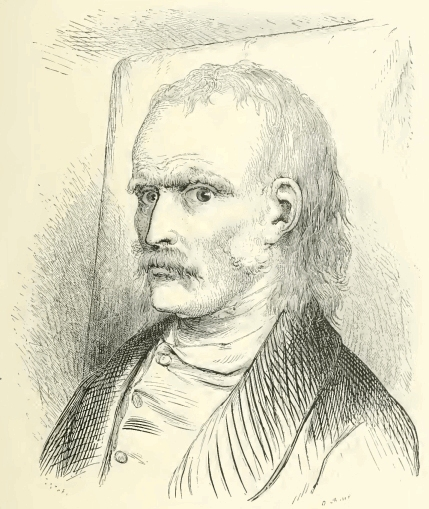
\includegraphics[width=\textwidth]{40046m.jpg}
\end{figure}

“Yes!”

“You!” cried Franz, whose hair stood on end; “you, M. Noirtier—you
killed my father?”

“Yes!” replied Noirtier, fixing a majestic look on the young man. Franz
fell powerless on a chair; Villefort opened the door and escaped, for
the idea had entered his mind to stifle the little remaining life in
the heart of this terrible old man.
